\documentclass[titlepage]{article}
\usepackage{polyglossia}
\usepackage{fontspec}
\setmainlanguage{russian}
\setmainfont{Times New Roman}
\usepackage{varwidth}
\usepackage{sectsty}
\usepackage{graphicx}
\usepackage[labelsep=endash]{caption}
\graphicspath{ {images/} }
\sectionfont{\centering}
\usepackage{geometry}
 \geometry{
 a4paper,
 total={170mm,257mm},
 left=20mm,
 top=20mm,
 }
\renewcommand{\labelitemi}{\textendash}
\newcommand{\goal}[1]{\textit{Цель работы:} #1}
\begin{document}
\captionsetup[figure]{name={Рисунок}}
\begin{titlepage}
\begin{center}
\MakeUppercase{Харьковский национальный университет радиоэлектроники}

\vspace*{\fill}
Отчет

по лабораторной работе №1

по теме "Моделирование задач многокритериального принятия решений"

\end{center}
\vspace{20mm}
\hfill
\begin{varwidth}{\linewidth}
Выполнили\\
ст. гр. ПЗСм-17-3\\
Гранкина Валерия\\
Гройс Михаил\\
Карачевцев Кирилл\\
Савченко Дмитрий\\

Проверила\\
доц. Мазурова О. А.
\end{varwidth}
\vspace*{\fill}

\centering{Харьков 2018}
\end{titlepage}
\goal{приобрести навыки использования и программной реализации средств информационной подготовки задач многокритериального принятия решений. Познакомиться с методами описания многокритериальных альтернатив, разных шкал оценивания альтернатив по критериям, методов нормирования оценок по разным типам шкал.}
\section*{Описание физической модели БД}

Физическая модель базы данных состоит из шести таблиц:
\begin{itemize}
\item Alternative --- таблица, которая содержит возможные альтернативы;
\item Criterion --- таблица критериев;
\item Mark --- таблица возможных оценок для каждого критерия;
\item Vector --- таблица, связывающая оценки и альтернативы;
\item LPR --- таблица с личностями, которые принимают решения;
\item Result --- таблица результатов.

Детальное описание схемы представлено на рисунке \ref{fig:schema}.

\begin{figure}[h]
\centering
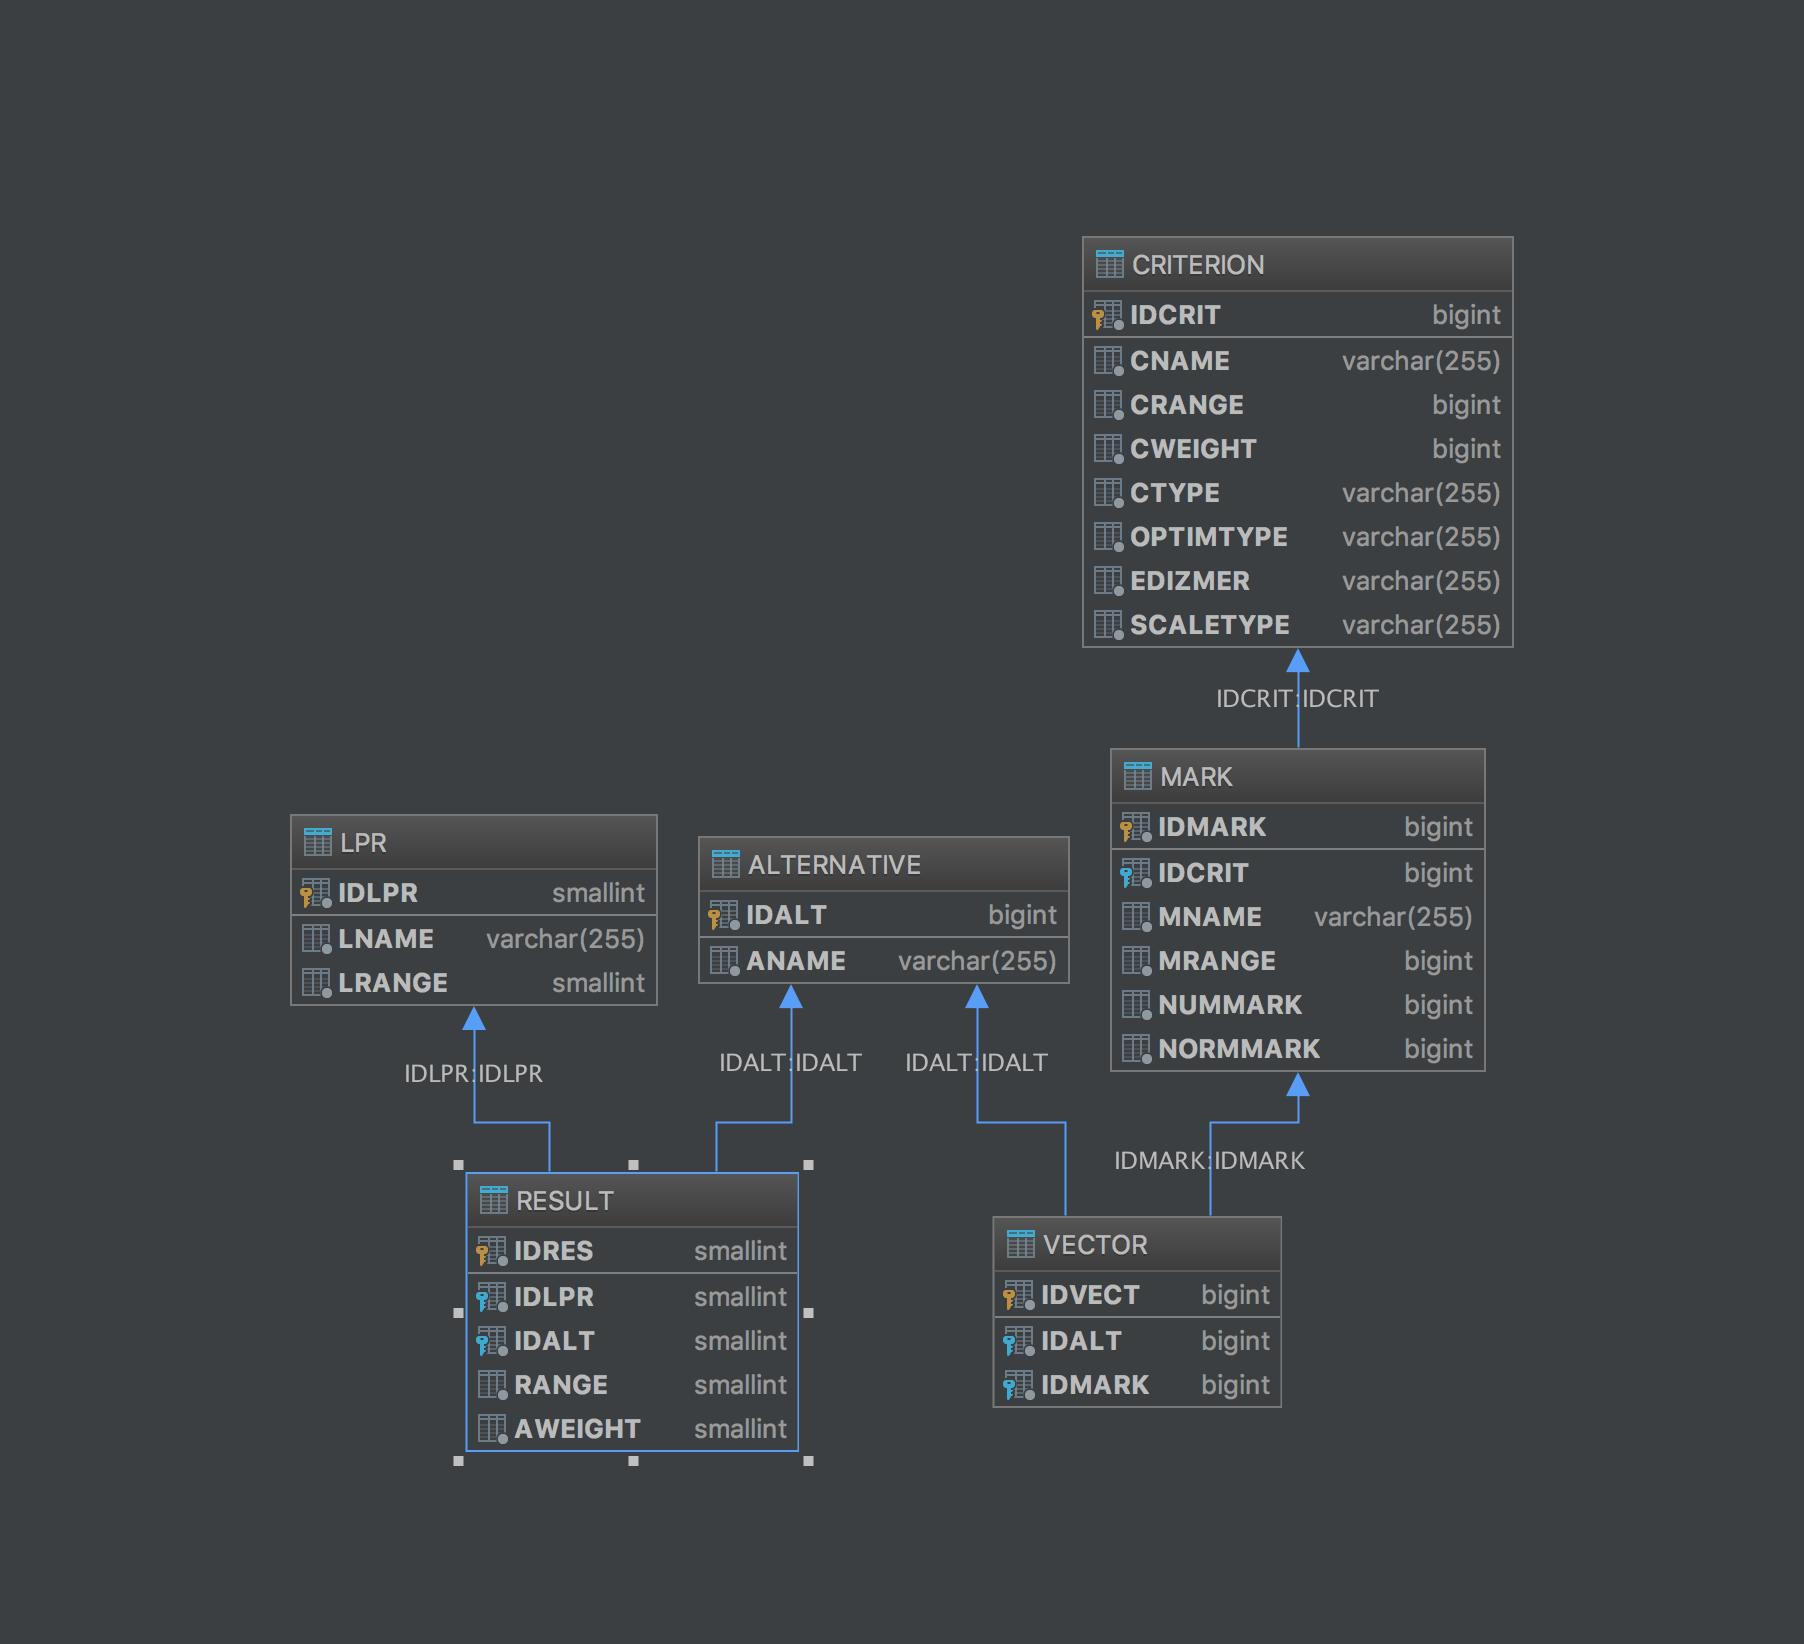
\includegraphics[scale=0.4]{schema}
\caption{Схема базы данных}
\label{fig:schema}
\end{figure}
\end{itemize}
\end{document}
